% Admir, Anna,  Sune (prototype)

% API implementation - Google, Firebase, Activity Recognition (Admir)
% Data Collection - Geofence, Activity Recognition, Location (Sune) - blir det ikke forklaret i section 5.2
% Search (Sune)
% Distance calculator
% ILocation and IStorage or other with interface and listener
% Adapter view pattern (Anna)

% TODO:
% Apply definitions
% Introduction
% Explain three different categories of prototyping
%    - Explorative, Experimental, Evoulutionary


In the following sections, central aspects of the Bikebus solution will be highlighted. This are applied examples on compression techniques and examples of architectural designs. 

% TODO:
% Explain all protoypes in our program (Implementation)
%    - Datastructures, algorithms, storage, etc
%    - Diagrams
%    - Results of prototypes

% Current Prototypes:
% - Easily shift sensor API (modifiability) 
%    - EmotionSenseLocation.java and ILocation  
% - SQLite for internal storage (availablity)


% Prototypes:
\section{Compression}
One of the features which needs to implemented in Bikebus is the compression functionality of locations points. Three prototypes have been made separate from the application which are illustrated in following examples. All examples are done in Python and plotted with Leaflet.  

Figure \ref{fig:route_without_filter} illustrates a clip of the raw data of a biking route. The route consists of 630 location points. On figure \ref{fig:route_with_filter} the median filter is applied on same route. By applying the median filter result in a much more smooth route, with less outliers/noise, which is described in section \ref{sec:data_processing}. 
\begin{figure}[H]
\centering
\begin{minipage}{0.50\textwidth}
\centering
    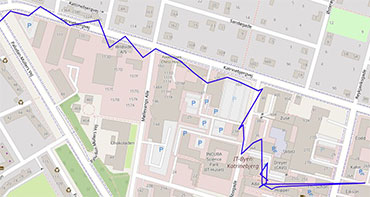
\includegraphics[width=\linewidth]{RouteWithOutFilter2.jpg}
    \caption{Without median filter}
    \label{fig:route_without_filter}
\end{minipage}\hfill
\begin{minipage}{0.50\textwidth}
\centering
    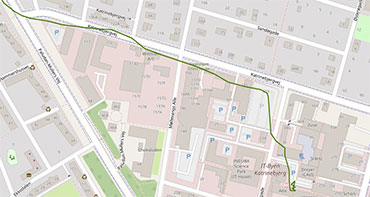
\includegraphics[width=\linewidth]{RouteWithFilter2.jpg}
    \caption{With median filter}
    \label{fig:route_with_filter}
\end{minipage}
\end{figure}

To get a better overview, both of the following maps are rotated. The DP compression is applied on figure \ref{fig:douglas_peucker_compression}. After applying the DP the routes is compressed to 20 location points. Figure \ref{fig:sliding_window} shows the route after applying Sliding window. For this prototype the code simulates how location points arrives periodically to be processed by the Sliding window algorithm. The compression results in 304 location points, which is $50\%$ compression of the original route.

\begin{figure}[H]
\centering
\begin{minipage}{0.50\textwidth}
\centering
    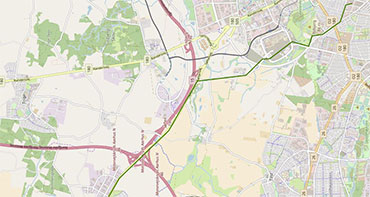
\includegraphics[width=\linewidth]{RouteDP2.jpg}
    \caption{Douglas Peucker compression (offline)}
    \label{fig:douglas_peucker_compression}
\end{minipage}\hfill
\begin{minipage}{0.50\textwidth}
\centering
    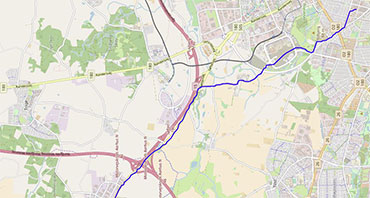
\includegraphics[width=\linewidth]{RouteSW2.jpg}
    \caption{Sliding window compression (online)}
    \label{fig:sliding_window}
\end{minipage}
\end{figure}

Since the core engine of Bikebus is build on a flexible architecture, it should be manageable to plug these algorithms into Bikebus. When pluggin compression algorithm into Bikebus more testing has to be done on how it affects the energy consumption. 

\section{Module viewpoint of the distance calculation}
By encapsulated the distance calculation, the system is robust to changes. The first implementation was the simple distance calculator which consist of a primitive euclidean distances calculation. Later when the Google API was integrated the Google distance matrix was implemented. By using a strategy pattern \cite{Baerbak10} it was easy to implement the new calculator without breaking existing functionality. 

\begin{figure}[H]
\centering
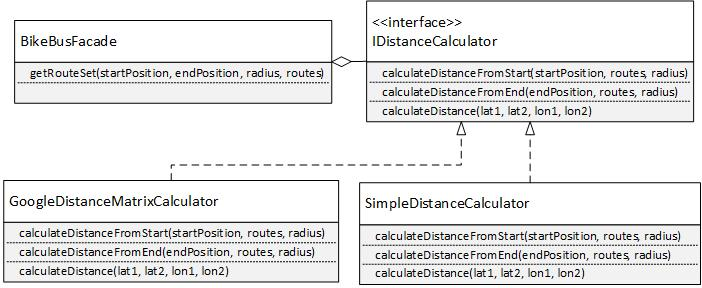
\includegraphics[scale=0.6]{Distance.jpg}
\caption{Module viewpoint of the strategy pattern of distance calculation}
\label{fig:module_view_distance_calculation}
\end{figure}

\section{Module viewpoint of the activity recognition and location}
As stated in section \ref{subsec:modifiability} the encapsulation tactic was chosen to achieve modifiability on replacing the sensor framework. The encapsulation is realized by coding to small interfaces and thereby achieving low coupling and high cohesion. Figure \ref{fig:activity_regonition_module_viewpoint} is a rough overview of the relations between the core classes gathering sensor data when biking.  
Notice that every class is encapsulated behind an interface. This also holds true for the activity recognition package seen in figure \ref{fig:Module_View_Sensor_Data}. It should be durable to hold the response measure by doing change by addition \cite{Baerbak10}.    

\begin{figure}[H]
\centering
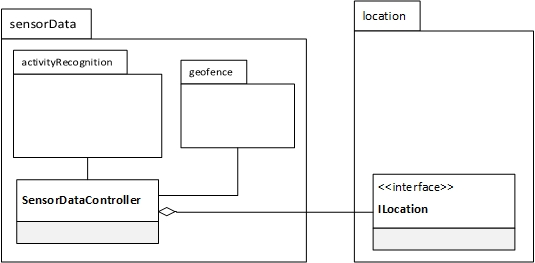
\includegraphics[scale=0.6]{ActivityRegonitionModuleViewpoint.jpg}
\caption{Module viewpoint of sensorData and location package}
\label{fig:activity_regonition_module_viewpoint}
\end{figure}